\documentclass{article}
\usepackage[utf8]{inputenc}
\usepackage{graphicx}
\graphicspath{ {./images/} }

\title{Weekly Assignment - As00 - BDSA}
\author{Malthe Mathias Mølgaard Larsen \\ malla@itu.dk }
\date{8. September 2021}

\begin{document}

\maketitle

\section{IsLeapYear Diagram}

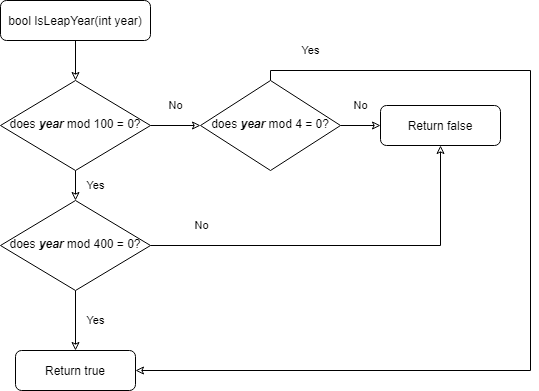
\includegraphics[scale=0.7]{images/LeapYearFlow.png}
\newpage
\section{IsLeapYear Description}
In the image above is the method \emph{IsLeapYear()} visualized. The method takes a year in the form of an integer as input, and returns true or false, depending on if the input is a leap year or not.\\
The method starts by checking if the inputted year modulus 100 is equal to 0, if this is true, there is another check to see if the year modulus 400 is equal to 0. If this is true, the method returns true and the inputted year is a leap year, if it is false, the method returns false and the year is not a leap year. \\
If however the first check for the year modulus 100 being equal to 0 is false, the year modulus 4 = 0 will be checked. If this is true, the method will return true, and the year is a leap year, if it is false it will return false, and the year is not a leap year.

\end{document}